\documentclass{beamer}
\usetheme{Warsaw}

\usepackage[utf8]{inputenc}
\usepackage{fancybox}
\usepackage{multimedia} 
\usepackage{subfig}
\usepackage{amsmath}
\usepackage{hyperref}
\usepackage[all]{xy}
\begin{document}


\title[Stochastik] % (optional, only for long titles)
{Stochastik für Informatiker
\\
\includegraphics[scale=0.5]{img/craps}
}
\subtitle{}
\author[Dr. Johannes Riesterer] % (optional, for multiple authors)
{Dr.  rer. nat. Johannes Riesterer}

\date[KPT 2004] % (optional)
{}

\subject{Stochastik}


\frame{\titlepage}


\begin{frame}
    \frametitle{Zufallsvariablen}
\framesubtitle{}

\begin{block}{Messraum}
Ein Messraum ist ein Paar $(\Omega, \mathcal{A})$ bestehend aus einer Menge $\Omega$ und einer Sigma-Algebra $\mathcal{A} \subset \mathcal{P}(\Omega)$.
\end{block}

\begin{block}{Zufallsvariablen}
Sei $(\Omega, \mathcal{A}, P)$ ein Wahrscheinlichkeitsraum und $(\Omega', \mathcal{A}')$ ein Messraum. Eine Zufallsvariable ist eine Abbildung
$$X : \Omega \to \Omega'$$ 
so dass für alle Ereignisse $A' \in  \mathcal{A}'$
$$ X^{-1} (A') \in \mathcal{A}$$
 ein Ereignis in $\mathcal{A}$ ist. Urbilder von Ereignissen sind also Ereignisse.
\end{block}

 \end{frame}

\begin{frame}
    \frametitle{Zufallsvariablen}
\framesubtitle{}
\begin{block}{Beispiel (Münzwurf)}
$\Omega = \{\text{Kopf}, \text{Zahl} \} $, $R = \{ 0,1 \}$  mit jeweils Potenzmenge als Sigma-Algebra und 
\begin{align*}
& X (\text{Kopf} ) = 0 \\
& X (\text{Zahl} ) = 1 
\end{align*}
\end{block}

\begin{block}{Beispiel (Summe zweier Würfel)}
$\Omega = \{1,2,3,4,5,6 \} \times \{1,2,3,4,5,6 \} $, $R = \{ 2,3,4,5,6,7,8,9,10, 11, 12\}$   mit jeweils Potenzmenge als Sigma-Algebra und $X: \Omega \to R; X (a,b) := a +b$. 
\end{block}

 \end{frame}

\begin{frame}
    \frametitle{Zufallsvariablen}
\framesubtitle{}
\begin{block}{Bildmaß}
Sei $(\Omega, \mathcal{A}, P)$ ein Wahrscheinlichkeitsraum, $(\Omega', \mathcal{A}')$ ein Messraum und  $X : \Omega \to \Omega'$  Eine Zufallsvariable. 
Durch 
\begin{align*}
P_X (A') := P(X^{-1} (A))
\end{align*}
 für $A' \in \mathcal{A}'$ wird ein Wahrscheinlichkeitsmaß auf  $(\Omega', \mathcal{A}')$ definiert. Es wird Bildmaß genannt. Anstelle von $P_X (A')$ wird auch die Schreibweise $P (X \in A'):= P_X (A')$ verwendet.
\end{block}


 \end{frame}

\begin{frame}
    \frametitle{Zufallsvariablen}
\framesubtitle{}

\begin{block}{Beispiel (Summe zweier Würfel)}
$\Omega = \{1,2,3,4,5,6 \} \times \{1,2,3,4,5,6 \} $, $R = \{ 2,3,4,5,6,7,8,9,10, 11, 12\}$ und $X: \Omega \to R; X (a,b) := a +b$. Dann ist 
$P_X(3) = P((1,2), (2,1)) = \frac{2}{36} = \frac{1}{18}$ 
\end{block}

 \end{frame}




\begin{frame}
    \frametitle{Integration bezüglich eine WMaßes}
\framesubtitle{}

\begin{block}{Indikatorfunktion}
Für eine Teilmenge $A \in \mathcal{A}$ heißt
$$ 1_A (x): = \begin{cases} 1 \text{  falls }   x \in A  \\  0  \text{  sonst}  \end{cases}$$
Indikatorfunktion.
\end{block}

\begin{block}{}
Eine Funktion 
$$ \varphi(x) := \sum_{k=1}^m c_k 1_{A_k}$$ mit $c_k \in \mathbb{R}$ und $A_k \in \mathcal{A}$ mit $A_i \cap A_j = \emptyset$ für $i \neq j$
heißt Treppenfunktion.
\end{block}

 \end{frame}


\begin{frame}
    \frametitle{Integration bezüglich eine WMaßes}
\framesubtitle{}

\begin{block}{Hüllreihe}
Eine Hüllreihe zu einer Funktion $f :\Omega \to \mathbb{R}$ ist eine Reihe $\phi(x):= \sum_{k=1}^{\infty} c_k  1_{A_k} (x)$ mit den folgenden Eigenschaften:
\begin{itemize}
\item $c_k \in \mathbb{R}$ sind positive reelle Zahlen $c_k >0$.
\item $A_k \subset \mathcal{A}$.
\item Für alle $x \in \Omega$ gilt $|f(x) | \leq \phi(x)$.
\end{itemize}
\end{block}

 \end{frame}



\begin{frame}
    \frametitle{Integration bezüglich eine WMaßes}
\framesubtitle{}

\begin{block}{}
Für eine Treppenfunktion $ \varphi(x) := \sum_{k=1}^m c_k 1_{A_k}$ definieren wir das Integral durch
$$\int_{\mathbb{R}^n} \varphi dP := \sum_{k =1}^m  c_k P(A_k) \; . $$
\end{block}


\begin{block}{}
Der Innhalt einer Hüllreihe $\phi(x):= \sum_{k=1}^{\infty} c_k  1_{A_k} (x)$ ist definiert durch 
$$I_P (\phi) := \sum_{k=1}^{\infty} c_k \;  P(A_k) \; .$$
\end{block}

 \end{frame}




\begin{frame}
    \frametitle{Integration bezüglich eine WMaßes}
\framesubtitle{}

\begin{block}{}
Die $L_{P^1}$-Halbnorm einer Funktion $f : \Omega\to \mathbb{R}$ is definiert durch das Infimum der Inhalte der Hüllreihen zu $f$
$$ || f ||_{P^1} : = \inf  \biggl \{   I(\phi) \; | \; \phi  \text{ ist Hüllreihe zu  }  f \biggr \} \; .$$
\end{block}

\begin{block}{}
Eine Funktion $f : \Omega \to \mathbb{R}$ heißt integrierbar, falls eine Folge von Treppenfunktionen  $\varphi_k$ existiert mit
$$ || f -  \varphi_k ||_1 \to 0 \text{ für } k \to \infty \;. $$
In diesem Fall heißt
$$ \int_{\mathbb{R}^n} f(x) dP := \lim_{k \to \infty}  \int_{\mathbb{R}^n}  \varphi_k d dP$$
das Integral von $f$ über $\mathbb{R}^n$.
\end{block}

 \end{frame}



\begin{frame}
    \frametitle{Integration bezüglich eine WMaßes}
\framesubtitle{}

\begin{block}{Neuer Wein in alten Schläuchen}
Integration bezüglich eines Wahrscheinlichkeitsmaßes Maßes verhält sich analog zu Lebesguemaß von letztem Semester.
\end{block}

 \end{frame}


\begin{frame}
    \frametitle{Reelle Zufallsvariablen}
\framesubtitle{}

\begin{block}{}
Eine Menge $U \subset  \mathbb{R}^n$ heißt offen, falls für jeden Punkt $x \in U$ ein Radius $\epsilon > 0$ existiert, so dass der Ball $B_\epsilon (x)$ in $U$ enthalten ist, also 
$B_\epsilon (x) \subset U$ gilt.
\end{block}

\begin{figure}[htp]
      \centering
    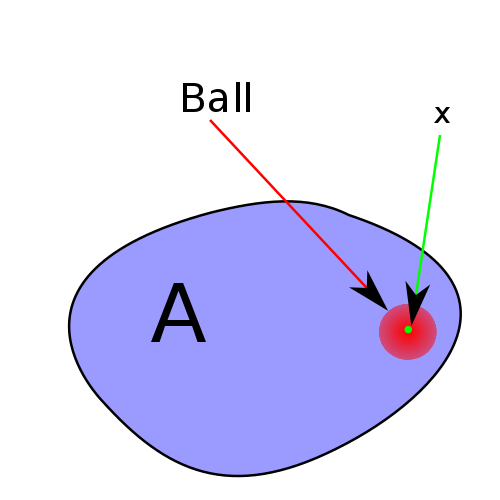
\includegraphics[width=0.45\textwidth]{img/openset}
      \caption{Quelle: Wikipedia}
\end{figure}


 \end{frame}


\begin{frame}
    \frametitle{Zufallsvariablen}
\framesubtitle{}

\begin{block}{Borell'sche Sigma-Algebra}
Die Borel'sche   $\sigma$-Algebra $\mathcal{B}(\mathbb{R}^n)$über $\mathbb{R}^n$ ist die kleinste  $\sigma$-Algebra, die alle offenen Mengen $\mathcal{U}$ enthält, also 
\begin{align*}
A_\sigma (\mathcal{U}) := \bigcap \{  \mathcal{A} \subset \mathcal{P}(\mathbb{R}^n);  \;   \mathcal{U}  \subset  \mathcal{A},  \;  \mathcal{A} \text{ ist $\sigma$-Algebra} \}
\end{align*}
\end{block}

\begin{block}{Existenz}
Die Borel'sche   $\sigma$-Algebra existiert, da die Potenzmenge eine   $\sigma$-Algebra ist.
\end{block}

\begin{block}{Messbarkeit}
Die Borel'sche   $\sigma$-Algebra ist in der $\sigma$-Algebra der Lebesgue messbaren Mengen enthalten.
\end{block}
 \end{frame}





\begin{frame}
    \frametitle{Zufallsvariablen}
\framesubtitle{}

\begin{block}{Reelle Zufalssvariable}
Unter einer reellen Zufallsvariable verstehen wir eine Zufallsvariable 
\begin{align*}
& X : \Omega \to \mathbb{R}^n \\
& X(\omega) := \biggl(X_1(\omega), \cdots , X_n(\omega)  \biggr) \; ,
\end{align*}
wobei $(\Omega, \mathcal{A}, P)$ ein Wahrscheinlichkeitsraum ist und $(\mathbb{R}^n, \mathcal{B}(\mathbb{R}^n)$ der $\mathbb{R}^n$ zusammen mit der Borell'schen Sigma-Algebra ist. Das Integral ist komponentenweise definiert durch
\begin{align*} 
\int_{\Omega} X dP :=  \biggl( \int_{\Omega} X_1 dP, \cdots , \int_{\Omega} X_n dP    \biggr)
\end{align*}

\end{block}

 \end{frame}


\end{document}
